%%%%%%%%%%%%%%%%%%%%%%%%%%%%%%%%%%%%%%%%%
% Journal Article
% LaTeX Template
% Version 1.4 (15/5/16)
%
% This template has been downloaded from:
% http://www.LaTeXTemplates.com
%
% Original author:
% Frits Wenneker (http://www.howtotex.com) with extensive modifications by
% Vel (vel@LaTeXTemplates.com)
%
% License:
% CC BY-NC-SA 3.0 (http://creativecommons.org/licenses/by-nc-sa/3.0/)
%
%%%%%%%%%%%%%%%%%%%%%%%%%%%%%%%%%%%%%%%%%

%----------------------------------------------------------------------------------------
%	PACKAGES AND OTHER DOCUMENT CONFIGURATIONS
%----------------------------------------------------------------------------------------

\documentclass[twoside,twocolumn]{article}

\usepackage{blindtext} % Package to generate dummy text throughout this template 

\usepackage[sc]{mathpazo} % Use the Palatino font
\usepackage{lmodern} % Czy nie usunąć? Może lepiej wygląda bez
\usepackage[utf8]{inputenc}
\usepackage[T1]{fontenc} % Use 8-bit encoding that has 256 glyphs
\linespread{1.05} % Line spacing - Palatino needs more space between lines
\usepackage{microtype} % Slightly tweak font spacing for aesthetics

\usepackage[polish]{babel} % Language hyphenation and typographical rules
\usepackage{polski}

\usepackage[hmarginratio=1:1,top=32mm,columnsep=20pt]{geometry} % Document margins
\usepackage[hang, small,labelfont=bf,up,textfont=it,up]{caption} % Custom captions under/above floats in tables or figures
\usepackage{booktabs} % Horizontal rules in tables

\usepackage{lettrine} % The lettrine is the first enlarged letter at the beginning of the text

\usepackage{enumitem} % Customized lists
\setlist[itemize]{noitemsep} % Make itemize lists more compact

\usepackage{abstract} % Allows abstract customization
\renewcommand{\abstractnamefont}{\normalfont\bfseries} % Set the "Abstract" text to bold
\renewcommand{\abstracttextfont}{\normalfont\small\itshape} % Set the abstract itself to small italic text

\usepackage{titlesec} % Allows customization of titles
\renewcommand\thesection{\Roman{section}} % Roman numerals for the sections
\renewcommand\thesubsection{\roman{subsection}} % roman numerals for subsections
\titleformat{\section}[block]{\large\scshape\centering}{\thesection.}{1em}{} % Change the look of the section titles
\titleformat{\subsection}[block]{\large}{\thesubsection.}{1em}{} % Change the look of the section titles

\usepackage{fancyhdr} % Headers and footers
\pagestyle{fancy} % All pages have headers and footers
\fancyhead{} % Blank out the default header
\fancyfoot{} % Blank out the default footer
\fancyhead[C]{ NBA $\bullet$ Grudzień 2018 } % Custom header text
\fancyfoot[RO,LE]{\thepage} % Custom footer text

\usepackage{titling} % Customizing the title section

\usepackage{hyperref} % For hyperlinks in the PDF

\usepackage{array}
\usepackage{graphicx}
\usepackage{subcaption}
\usepackage{multirow}

\usepackage{enumitem}
\newenvironment{nscenter}
 {\parskip=0pt\par\nopagebreak\centering}
 {\par\noindent\ignorespacesafterend}
%----------------------------------------------------------------------------------------
%	TITLE SECTION
%----------------------------------------------------------------------------------------

\setlength{\droptitle}{-4\baselineskip} % Move the title up

\pretitle{\begin{center}\Huge\bfseries} % Article title formatting
\posttitle{\end{center}} % Article title closing formatting
\title{Zastosowanie technik zgłębiania danych w przewidywaniu pozycji gracza NBA} % Article title
\author{%
\textsc{Jan Iwaszkiewicz}\thanks{indeks: 238215, kontakt: \href{mailto:jiwaszkiewicz6@gmail.com}{jiwaszkiewicz6@gmail.com}} \\[1ex] % Your name
\normalsize Uniwersytet Gdański \\ % Your institution
%\and % Uncomment if 2 authors are required, duplicate these 4 lines if more
%\textsc{Jane Smith}\thanks{Corresponding author} \\[1ex] % Second author's name
%\normalsize University of Utah \\ % Second author's institution
%\normalsize \href{mailto:jane@smith.com}{jane@smith.com} % Second author's email address
}
\date{\today} % Leave empty to omit a date
\renewcommand{\maketitlehookd}{%
\begin{abstract}
\noindent W poniższym opracowaniu przedstawione zostają klasyfikatory oraz inne metody zgłębiania danych pozwalające na określanie pozycji gracza ligi NBA. Przy wykorzystaniu statystyk z danego sezonu sprawdzona zostaje skuteczność przedstawionych algorytmów. Dodatkowo zostaje opisany sposób doboru danych oraz ich potencjalny wpływ na wyniki badań. % \blindtext % Dummy abstract text - replace \blindtext with your abstract text
\end{abstract}
}

%----------------------------------------------------------------------------------------

\begin{document}

% Print the title
\maketitle

%----------------------------------------------------------------------------------------
%	ARTICLE CONTENTS
%----------------------------------------------------------------------------------------

\section{Wstęp - opis bazy}

\lettrine[nindent=0em,lines=3]NBA to amerykańska liga koszykówki mężczyzn, najbardziej znana i dochodowa na świecie. Swój suckes zawdzięcza ciągłemu rozwojowi i dostosowywaniu się do potrzeb fanów sportu. Idzie za tym rozwój samych graczy, którzy muszą co wieczór zapewniać najwyższy poziom rozrywki. Od sportu dla studentów i amatorów do światowego widowiska najwyższej klasy, od ,,białego'' do ,,czarnego'' sportu - tak można opisać rozwój koszykówki oraz NBA. Celem przeprowadzonego eksperymentu będzie sprawdzenie, czy w danym roku możliwe jest sklasyfikowanie pozycji gracza na boisku. Zgodnie z założeniami sportu niektóre pozycje jak rozgrywający (Point Guard) czy środkowy (Center), mają znacząco różniące się zadania podczas rozgrywki. Idące za tym różnice w statystykach graczy powinny jasno wyznaczać poszczególne pozycje jako klasy. Czy na pewno?
%------------------------------------------------

\section{Przygotowanie danych}
\subsection{Czy sezon ma znaczenie?}
By w pełni wykorzystać bazę danych konieczne jest przygotowanie jej pod wymagane przez algorytmy dane wejściowe. Na początku projektu założone zostało, że rok 1980 zostanie najstarszym możliwym do wybrania rokiem. Dlaczego? W tym roku dopiero wprowadzono linię rzutów za 3 punkty oraz rozpoczęto prowadzenie szczegółowych statystyk podczas sezonu. Wcześniej nie prowadzono takowych ze względów technicznych oraz słabego zainteresowania sportem. Zatem jaki rok wybrano do badań? Tutaj wybór padł na 2017. Oprócz dokładnych statystyk, ważnym czynnikiem jest stan ligi. Sport ciągle ewoluuje, a mniej więcej od roku 2015 NBA przeżyło ogromne zmiany. Zaczęto wykorzystywać skutecznie linię rzutu za 3 punkty oraz pojawiło się dużo graczy ,,hybrydowych'', którzy nie są typowi dla swoich pozycji. Często są na tyle uniwersalni, że grają na pozycji, która aktualnie jest ważna dla danego zespołu lub dzięki temu uzysukją niesamowitą przewagę (przykładowo wzrostu) nad innymi graczami. Ostatecznie do badań wykorzystuje się jedynie jeden sezon. Dysproporcje między statystykami różnych sezonów mogą być na tyle duże, że określenie klasy będzie wręcz niemożliwe. Przykładem może być rok 1980 oraz 2016, gdzie w pierwszym oddawnano rzuty za 3 punkty okazyjnie w ostateczności, natomiast w drugim stało się to jednym z podstawowych elementów gry. 
\subsection{Statystyki danego gracza}
Wybrane bazy połączono i wykonano na nich odpowiednie operacje, by uzyskać następujące statystki:
\begin{itemize}
\item \textbf{Player}\\
Imię i nazwisko gracza, przycięte o niepotrzebne znaki.
\item \textbf{Height}\\
Wzrost gracza, podany w centymetrach.
\item \textbf{Weight}\\
Waga gracza, podana w kilogramach.
\item \textbf{PTSavg}\\
Średnia punktów z sezonu, ilość punktów ogółem podzielona na ilość rozegranych meczy.
\item \textbf{TRBavg}\\
Średnia zbiórek z sezonu, ilość zbiórek ogółem podzielona na ilość rozegranych meczy.
\item \textbf{ASTavg}\\
Średnia asyst z sezonu, ilość asyst ogółem podzielona na ilość rozegranych meczy.
\item \textbf{STLavg}\\
Średnia przechwytów z sezonu, ilość przechwytów ogółem podzielona na ilość rozegranych meczy.
\item \textbf{BLKavg}\\
Średnia bloków z sezonu, ilość bloków ogółem podzielona na ilość rozegranych meczy.
\item \textbf{TOVavg}\\
Średnia strat z sezonu, ilość strat ogółem podzielona na ilość rozegranych meczy.
\item \textbf{TS.}\\
True shooting precentage, statystka prowadzona by dokładniej określić skuteczność w oddawaniu rzutów.
\item \textbf{FG.}\\
Field goals precentage, skuteczność rzutów z gry.
\item \textbf{X3P.}\\
Skuteczność rzutów za 3 punkty.
\item \textbf{X2P.}\\
Skuteczność rzutów za 2 punkty.
\item \textbf{eFG.}\\
Effective field goal percentage, poprawiona statystyka z uwagą na ,,wartość'' rzutu (3 oraz 2 punkty).
\item \textbf{FT.}\\
Skuteczność rzutów z linii rzutów osobistych.
\item \textbf{Pos}\\
Pozycja gracza na boisku, w wypadku wielu pozycji (gdy gracz w jednym sezonie przechodził między drużynami) wybrana zostaje pozycja na której rozegrał najwięcej spotkań.
\end{itemize}
Wszystkie statystki zostają dodatkowo wyselekcjonowane, bądź poddane innym operacjom w wypadku korzystania z poszczególnych algorytmów. Przy wystąpieniu wartości niemożliwych do zdefiniowania NA lub -INF, dane zastępowano średnimi ligowymi, bądź zerami w zależności od potrzeb.
\subsection{Pozycja na boisku jako klasa}
By możliwe ułatwić pracę oraz dopasować się do założeń projektu kolumna z pozycją gracza upraszcza się do decyzji ,,yes'' lub ,,no''. Pozycję którą chcemy poddać klasyfikacji ustalamy za pomocą zmiennej ,,desired position''. Dostępne prametry to ,,PG'', ,,SG'', ,,SF'', ,,PF'' oraz ,,C''.
%------------------------------------------------

\section{Klasyfikatory}
\subsection{Podział na zbiory}
\indent Do klasyfikatorów C4.5/ID3 (drzewo), Naive Bayes, kNN niezbędny jest podział danych na zbiory treningowe i testowe. Dokonano go za pomocą losowego wybrania rekordów przy prawdopodobieństawch 67\% oraz 33\%. Do metody kNN znormalizowane zostały również wszystkie kolumny z wartościami numerycznymi.
\newpage
\subsection{Porównanie klasyfikatorów}
\indent Na przygotowanej bazie dokonano klasyfikacji za pomocą następujących metod.
\begin{itemize}
\item \textbf{C4.5/ID3 - drzewo decyzyjne}
\item \textbf{Naive Bayes}
\item \textbf{kNN - k najbliższych sąsiadów}
Przy użyciu dwóch najbliższych sąsiadów.
\item \textbf{Hierarchical Clustering}
Metoda pokrewna do k-średnich. Jednak wykazująca większą skuteczność dla wybranej bazy.
\end{itemize}

Oprócz wymienionych metod do wykresu przedstawiającego skuteczność klasyfikacji, zestawiona została również metoda k-Means. Pozwala to porównać ją z pochodzącym z tej samej rodziny sposobem Hierarchical Clustering. Wyniki widoczne są na Rysunku 1. Wyznaczone zastały również macierze błędu dla metod (Tablice 1, 2, 3 oraz 4). Przeprowadzone poza zakresem sprawozdania testy zwracały podobne wyniki dla większości sezonów, poza okresem (1996-2000) dla pozycji PG gdzie dochodziło do spadku skuteczności. Również pozycje ,,bardziej płynne'' (SG, SF, PF), które często są wymienne i mają średnie statystki zbliżone do siebie, wykazywały się niższą skutecznością klasyfikacji. Szczególnie widoczne jest to w ,,nowoczesnej erze'' NBA, rozpoczynającej się od połowy lat 90, aż do niedawno zanotowanego sezonu 2017.
\begin{figure}[hbt!]
  \centering
    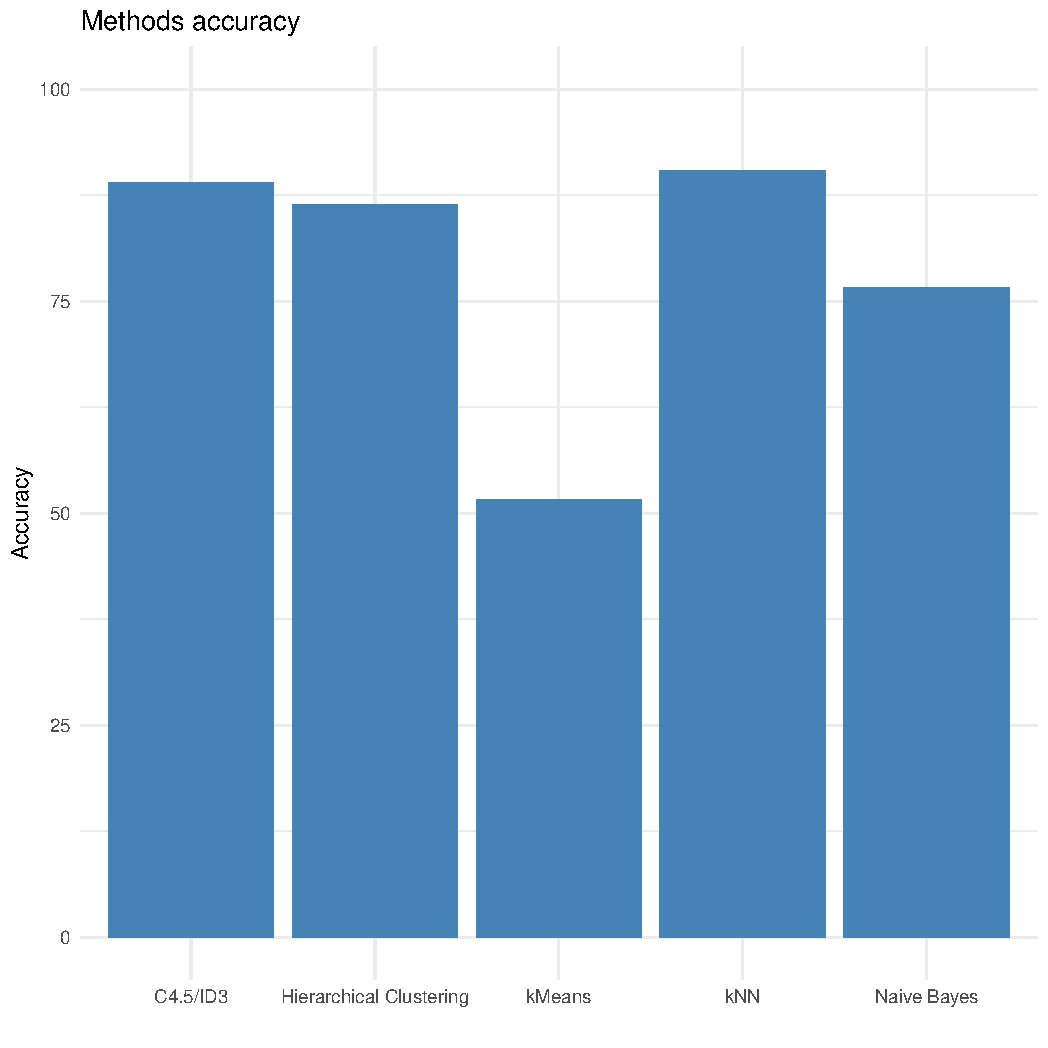
\includegraphics[width=\linewidth]{plot_acc.pdf}
  \caption{Porówanie skuteczności w klasyfikowaniu graczy dla pozycji PG na podstawie danych z roku 2017.}
  \label{fig:coffee}
\end{figure}

\begin{table}[hbt!]
\centering
\caption{Macierz błędu : C4.5/ID3 - drzewo decyzyjne}
\begin{tabular}{l*{2}{c}r}
Pred/Real & no & yes \\
\hline
no & 118 & 9 \\
yes & 8 & 19 \\
\end{tabular}
\end{table}

\begin{table}[hbt!]
\centering
\caption{Macierz błędu : Naive Bayes}
\begin{tabular}{l*{2}{c}r}
Pred/Real & no & yes \\
\hline
no & 97 & 7 \\
yes & 29 & 21 \\
\end{tabular}
\end{table}

\begin{table}[hbt!]
\centering
\caption{Macierz błędu : kNN - k najbliższych sąsiadów}
\begin{tabular}{l*{2}{c}r}
Pred/Real & no & yes \\
\hline
no & 114 & 7 \\
yes & 7 & 19 \\
\end{tabular}
\end{table}

\begin{table}[hbt!]
\centering
\caption{Macierz błędu : Hierarchical Clustering}
\begin{tabular}{l*{2}{c}r}
Pred/Real & no & yes \\
\hline
no & 342 & 18 \\
yes & 48 & 78 \\
\end{tabular}
\end{table}

\subsection{TP, FP, TN, FN, THC, TPR, FPR, NBA, UG i inne skróty}
Wartości TP, FP, TN, FN odpowiadają odpowiednio Prawdziwie Pozytywnemu, Fałszywie Pozytywnemu, Prawdziwie Negatywnemu oraz Fałszywie Negatywnemu zaklasyfikowaniu gracza na zadanej pozycji.
Wyliczone zostały również wartości TPR, FPR, FNR oraz TNR (znane jako sensitivity, fall-out, miss rate oraz specificity).
Zauważono również zależności między nimi:
\[ FPR + TNR = 1 \]
\[ TPR + FNR = 1 \]
\\
Wydzielono dwa rodzaje błędu:
\begin{itemize}
\item \textbf{Pierwszego rodzaju}\\
Czyli FP, błąd polegający na odrzuceniu hipotezy zerowej, która w rzeczywistości nie jest fałszywa.
\item \textbf{Drugiego rodzaju}\\
Oznaczony przez FN, błąd polegający na nieodrzuceniu hipotezy zerowej, która jest w rzeczywistości fałszywa.
\end{itemize}
Zakładamy, że szukamy  rozgrywających. Zatem TP odpowiada poprawnemu przydzielniu klasy yes dla gracza będącego na pozycji rozgrywającego, FP przydzieleniu klasy yes dla gracza występującego przykładowo jako niski skrzydłowy, TN przypisaniu no dla rzucającego obrońcy oraz FN przydzieleniu no dla gracza będącego rozgrywającym.
\\
Oba błędy mają wpływ na wynik czynników TPR, FPR, FNR i TNR. Obserwacje można wyciągnąć już ze wzorów (literatura ,,Sensitivity and specificity''). Poniżej jednak przedstawiona zostanie tabelka (Tablica 5) wyjaśniająca zależności:

\begin{table}[hbt!]
\centering
\caption{Zależności wynikające z błędów pierwszego i drugiego rodzaju}
\begin{tabular}{cc|c|c|c|c|l}
\cline{3-6}
& & \multicolumn{4}{ c| }{Wartość} \\ \cline{3-6}
& & TPR & FPR & FNR & TNR \\ \cline{1-6}
\multicolumn{1}{ |c  }{\multirow{2}{*}{FP} } &
\multicolumn{1}{ |c| }{$\uparrow$} & - & $\uparrow$ & - & $\downarrow$ &     \\ \cline{2-6}
\multicolumn{1}{ |c  }{}                        &
\multicolumn{1}{ |c| }{$\downarrow$} & - & $\downarrow$ & - & $\uparrow$ &     \\ \cline{1-6}
\multicolumn{1}{ |c  }{\multirow{2}{*}{FN} } &
\multicolumn{1}{ |c| }{$\uparrow$} & $\downarrow$ & - & $\uparrow$ & - \\ \cline{2-6}
\multicolumn{1}{ |c  }{}                        &
\multicolumn{1}{ |c| }{$\downarrow$} & $\uparrow$ & - & $\downarrow$ & - \\ \cline{1-6}
\end{tabular}
\end{table}

\indent Osobistym przemyśleniem jest stwierdzenie, że błąd drugiego rodzaju (FN) jest bardziej ,,krzywdzący'' dla obserwowanego zbioru danych. Zaklasyfikowany w ten sposób gracz (czyli w tym przypadku rozgrywający) nie jest najczęściej przygotowany do innej roli na boisku niż dowodzenia drużyną. Natomiast popularną metodą w dzisiejszej koszykówce jest wystawianie niskiego skrzydłowego jako rozgrywającego, który może w ten sposób rozciągnąć grę, jednocześnie posiadając podobny zestaw umiejętności co rozgrywający. Zatem błąd pierwszego rodzaju nie jest koniecznie krzywdzący, gdyby jakaś drużyna starała się dobierać gracza na podstawie wyników klasyfikatora.

\begin{figure}[hbt!]
  \centering
    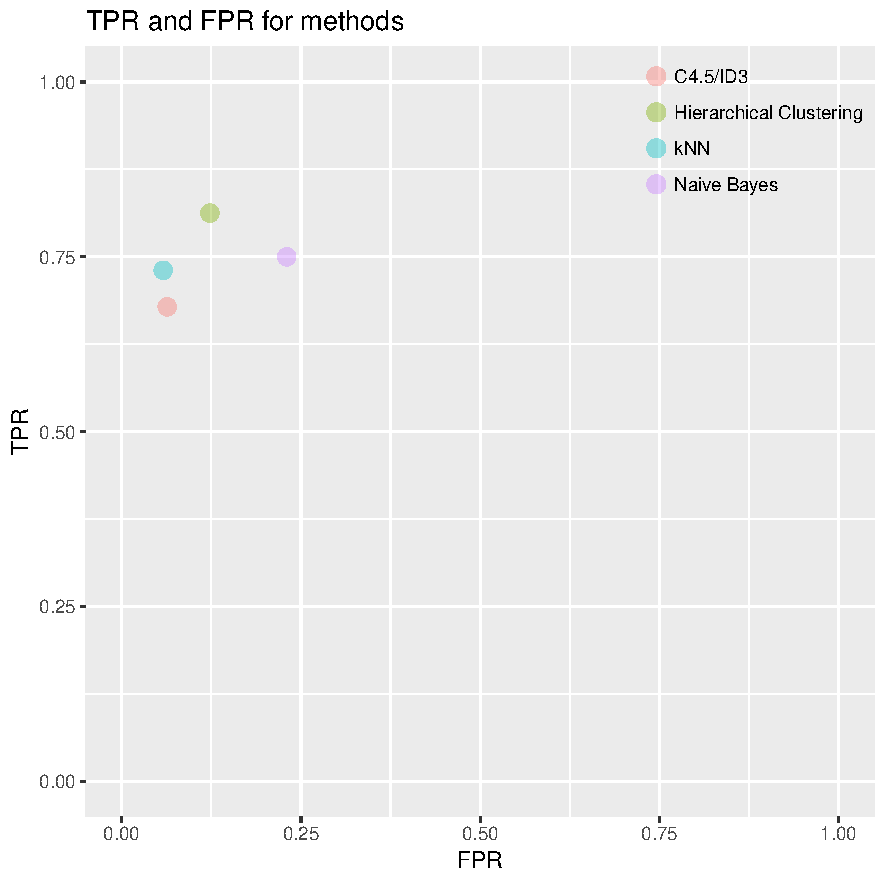
\includegraphics[width=\linewidth]{plot_ROCspace.pdf}
  \caption{Porównanie sensitivity i false alarm dla klasyfikatorów.}
  \label{fig:coffee}
\end{figure}

\indent Na wykresie (Rysunek 2) przedstawione jest położenie klasyfikatorów w zależności od wyników FPR i TPR. Zakładając, że najlepszy klasyfikator nie popełnia błędów, idealna sytuacja zachodzi przy braku błędów. Znaczy to, że FP i FN są równe 0. Wtedy wartość TPR równa się 1, natomiast FPR wynosi 0. Zatem najlepszy klasyfikator znajduje się w punkcie (x = 0, y = 1), mówiąc potoczniej - w lewej górnej części wykresu. Odległości poszczególnych klasyfikatorów zostały obliczone i porównane (Tablica 6).

\begin{table}[hbt!]
\centering
\caption{Odległość metody od współrzędnej (0,1) na Rysunku 2}
\begin{tabular}{l*{4}{c}}
Metoda & Odległość \\
\hline
Hierarchical Clustering & 0.2242859 \\
kNN & 0.2753761 \\
C4.5/ID3 & 0.3276394 \\
Naive Bayes & 0.3620692 \\
\end{tabular}
\end{table}
\newpage
\indent Jeżeli zwracamy uwagę jedynie na liczby najlepszym rozwiązaniem wydają się być Hierarchical Clustering oraz kNN, ponieważ znajdują się nabliżej założeń klasyfikatora idealnego. Jednak biorąc pod uwagę stabliność (szczególnie w innych latach) algorytm kNN lub C4.5/ID3 wydaje się być lepiej przystosowany do zadania.

%------------------------------------------------

\section{Grupowanie metodą k-średnich}

\subsection{Metoda nieskuteczna}

\indent Ze względu na naturę bazy metoda nie potrafiła osiągnąć pożądanych rezultatów. Klasa zazwyczaj jest niewyraźnie wydzielona od reszty oraz niewielka w stosunku do ogółu (zwyczajowo w sezonie 20\% zawodników jest odpowiednio przydzielonych do każdej z pozycji). Algorytm przedstawia się następująco (Rysunek 3). Widoczne centroidy dzielą ligę dokładnie w połowie. Inną możliwą przeszkodą, dla działania algorytmu, mogą być przeprowadzone operacje poprzedzające wprowadzenie danych wejściowych (log). Być może powodują zbyt duże znormalizowanie danych.

\begin{figure}[hbt!]
  \centering
    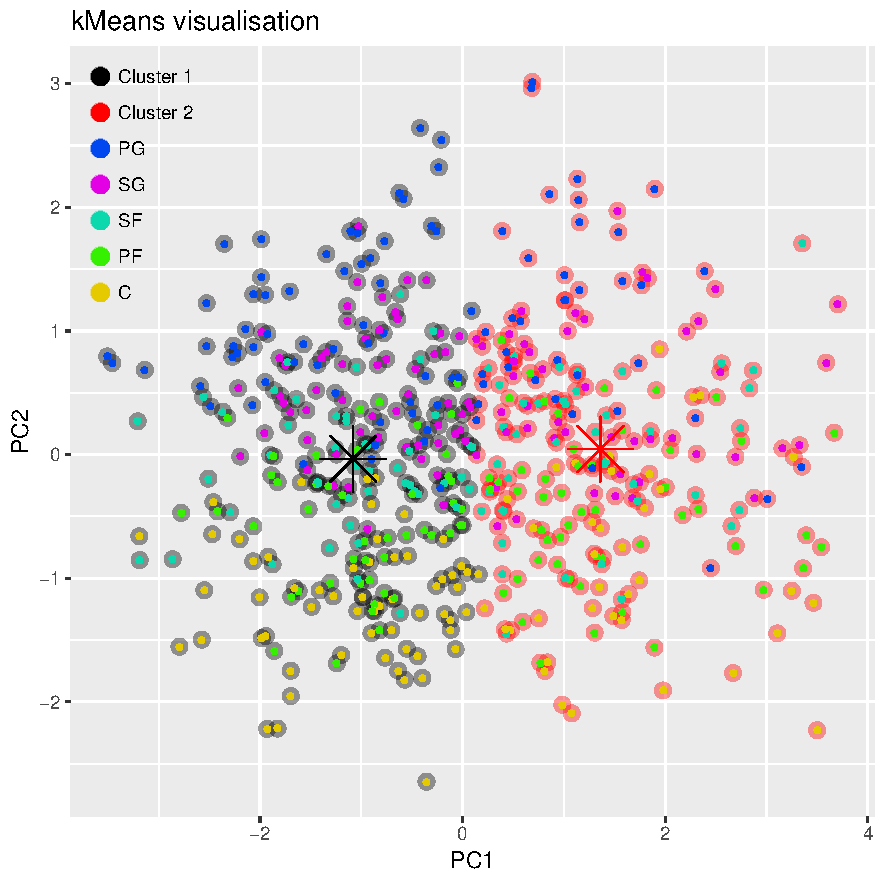
\includegraphics[width=\linewidth]{plot_kclust.pdf}
  \caption{Metoda k-średnich : klastry oraz nałożona na nią liga, sezon 2017.}
  \label{fig:coffee}
\end{figure}
\newpage
\subsection{Czy można to zrobić inaczej?}

\indent Obserwując wyniki metody k-means, postanowione zostało znaleźenie skutecznego rozwiązania dla problemu klastrowania. Wspomniane wcześniej Grupowanie Hierarchiczne (Hierarchical Clustering) opiera się na dzieleniu obserwacji na klastry bazując na podobieństwach między nimi. Nie jest tutaj konieczne określenie ilości klastrów na początku działania. Zatem bardzo możliwe wydaje się znalezienie dwóch grup, które z założeń projektu powinny być łatwe do wydzielenia ze zbioru obserwacji. Do obliczeń potrzebnych w algorytmie  skorzystano z metody Połączeń Ward'a pod nazwą ward.D2. Korzysta ona z obserwacji, dzięki której nie jest wymagane podniesienie do kwadratu wszystkich odchyleń od punktów do centroidów. W procesie tworzą się pary zawierające pojedyncze obserwacje. Następnie pary klastrów są sukcesywnie łączone, aż do momentu gdy wszystkie klastry zostaną scalone w duży klaster zawierający podobne obiekty. Wyniki przedstawione zostały na Rysunku 4. Algorytm deprymuje pokrewną metodę k-średnich oraz prezentuje skuteczność zbliżoną do pozostałych metod (Rysunek 1).

\begin{figure}[hbt!]
  \centering
    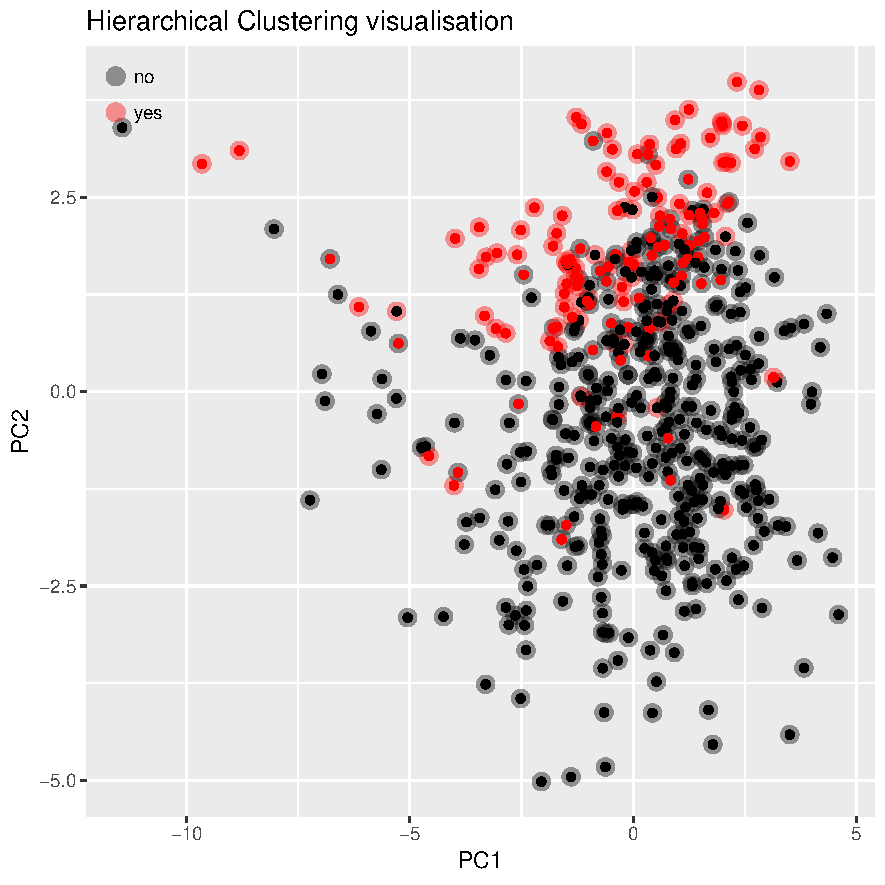
\includegraphics[width=\linewidth]{plot_hclust.pdf}
  \caption{Metoda Hierarchical Clustering : klastry oraz nałożona na nią liga, sezon 2017, pozycja PG.}
  \label{fig:coffee}
\end{figure}

%------------------------------------------------
\newpage
\section{Reguły asocjacyjne}

\indent Pomimo uproszczenia danych dwie wartości ,,above'', ,,bellow'' (powyżej i poniżej średnich ligowych) oraz wykluczeniu zbędnych lub powtarzających się, wyciągnięte z bazy reguły asocjacyjne można liczyć w setkach lub tysiącach. Wybrane zostały zatem tylko najbardziej interesujące z wysokim czynnikiem wiarygodności oraz wsparcia. Poniżej opisane kilka z nich:

\begin{itemize}
\item \textbf{Wynik: Pos=yes dla PG}\\
Zgodnie z założenieniami rozgrywający nie zdobywa wielu punktów oraz nie gra pod koszem przez swój wzrost i wagę (poniżej średniej Height, Weight, TRBavg oraz BLKavg). Opiera swoją grę na asystach i przechwytach. Odznacza się również dobrym \% z linii osobitych. Przykłady:
\begin{itemize}
	\item PTSavg=bellow \\ ASTavg=above\\ STLavg=above\\ BLKavg=bellow\\ X3P.=bellow \\ FT.=above \\
	\item Height=bellow \\ ASTavg=above \\ X3P.=bellow \\ FT.=above
\end{itemize}
\end{itemize}

\begin{itemize}
\item \textbf{Wynik: Pos=no dla PG}\\
Reguły dla pozostałych pozycji (najczęściej wyższych, silniejszych i grających bliżej kosza) również nie zaskoczyły podczas eksperymentu. Przykłady:
\begin{itemize}
	\item Height=above \\ Weight=above \\ TRBavg=above \\
	\item TRBavg=above \\ BLKavg=above \\ X3P.=bellow \\ FT.=above
\end{itemize}
\end{itemize}

%------------------------------------------------

\section{Podsumowanie badań}

\indent Po przeprowadzonych badaniach można zauważyć ewolucję koszykówki oraz graczy tworzących ligę NBA. Z biegiem czasu, różnice pomiędzy rolami na boisku coraz bardziej się zacierają. Nowe taktyki oraz wykorzystywanie statystyki w celu optymalizacji wyników drużyny, powodują drastyczne zmiany w założeniach koszykówki. W dniu dzisiejszym największą przeszkodą dla algorytmów jest uniwersalność obecnych w lidze zawodników. Jednak wciąż możliwe jest stosunkowo skuteczne sklasyfikowanie gracza, który odzacza się specjalną rolą na boisku (rozgrywający). Największym zaskoczeniem eksperymentu okazało się wykorzystanie innej niż przedstawionej podczas laboratoriów metody klasteryzacji. Pomimo swoich wad, przy odpowiednich danych, jest w stanie konkurować z innymi alogrytmami klasyfikującymi.

%----------------------------------------------------------------------------------------
%	REFERENCE LIST
%----------------------------------------------------------------------------------------

\begin{thebibliography}{99} % Bibliography - this is intentionally simple in this template

\bibitem[Zbiór danych]{b}
\newblock {\em NBA Players stats since 1950}, dostęp online:
\newblock \url{https://www.kaggle.com/drgilermo/nba-players-stats} 

\bibitem[Zasoby online]{a}
\newblock {\em Sensitivity and specificity }, dostęp online:
\newblock \url{https://en.wikipedia.org/wiki/Sensitivity_and_specificity}

\bibitem[Zasoby online]{b}
\newblock {\em How to understand the drawbacks of K-means }, dostęp online:
\newblock \url{https://stats.stackexchange.com/questions/133656/how-to-understand-the-drawbacks-of-k-means} 

\bibitem[Zasoby online]{b}
\newblock {\em Hierarchical Clustering }, dostęp online:
\newblock \url{https://en.wikipedia.org/wiki/Hierarchical_clustering} 

\bibitem[Fionn Murtagh, Pierre Legendre]{b}
\newblock {\em Ward’s Hierarchical Agglomerative Clustering Method:
Which Algorithms Implement Ward’s Criterion? }, dostęp online:
\newblock \url{hhttp://adn.biol.umontreal.ca/~numericalecology/Reprints/Murtagh_Legendre_J_Class_2014.pdf} 

\bibitem[Zasoby online]{b}
\newblock {\em Hierarchical Clustering documentation }, dostęp online:
\newblock \url{https://stat.ethz.ch/R-manual/R-devel/library/stats/html/hclust.html}
\end{thebibliography}

%----------------------------------------------------------------------------------------

\end{document}
